

\begin{figure}
\begin{subfigure}{.5\linewidth}
\centering

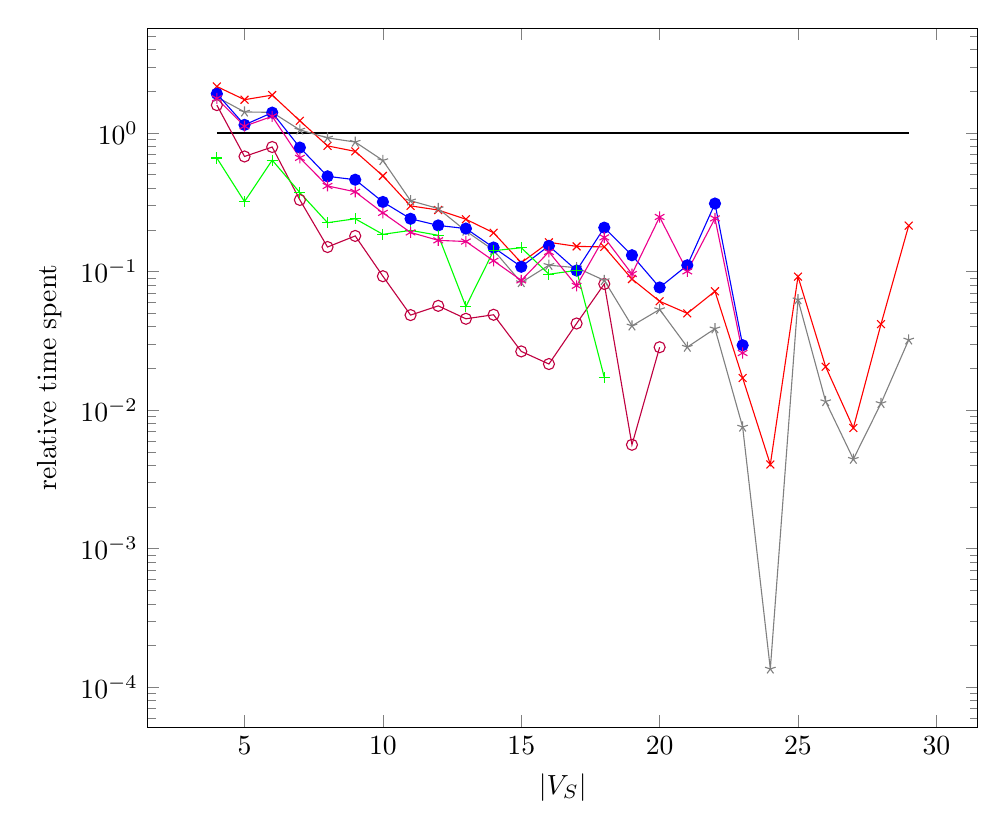
\begin{tikzpicture}
    \begin{axis}[
        xlabel=$|V_S|$,
        ylabel=relative time spent,
        ymode=log,
        legend style={at={(0.9,0.1)},anchor=south east},
        width=\textwidth,
		y tick label style={/pgf/number format/sci},
    ]


\addplot [mark=none, black] plot coordinates {
        (4,1) (29, 1)};
%\addlegendentry{No contraction}

	\addplot[
        mark=x,
        red,
    ] plot coordinates {
        (4,2.1674128912679387)
        (5,1.7391752267555143)
        (6,1.878677825130543)
        (7,1.2249805426145646)
        (8,0.8074738280349274)
        (9,0.7370517159428939)
        (10,0.4907351225256)
        (11,0.2980550454981918)
        (12,0.2781141325880348)
        (13,0.23851995177183047)
        (14,0.19062785566800405)
        (15,0.11582540953584422)
        (16,0.16268098061869612)
        (17,0.15207093622469334)
        (18,0.15064594752021512)
        (19,0.0883792576708712)
        (20,0.06105289023128585)
        (21,0.049964135000540935)
        (22,0.0721091008374441)
        (23,0.017061614763450757)
        (24,0.004054554777087193)
        (25,0.09203806626889509)
        (26,0.020561449567552532)
        (27,0.007440675118337155)
        (28,0.0417732163780968)
        (29,0.2146145702804488)
};
%    \addlegendentry{DFS}
%    \addplot[
%        mark=x,
%        red,
%    ] plot coordinates {
%        (4,1.764570104072358)
%        (5,1.2804472403537654)
%        (6,1.1184611822085426)
%        (7,1.108193754987779)
%        (8,1.0823455102636332)
%        (9,1.3202304844536292)
%        (10,0.8766301350767352)
%        (11,2.545919815002013)
%        (12,1.0352805568707166)
%        (13,0.7348584756068407)
%        (14,0.7849914287368015)
%        (15,0.8934474568976407)
%        (16,1.6666025961560895)
%        (17,0.71724791351521)
%        (18,0.5094398225741126)
%        (19,0.8456597164761079)
%        (20,0.8045735438552715)
%        (21,0.5994679253970462)
%        (22,0.4676165222586781)
%        (23,0.10986432258137258)
%        (24,0.16189794326161777)
%        (25,0.2926263173443996)
%        (26,0.09304326805518515)
%        (27,0.042335345258718515)
%        (28,0.1650463503335008)
%        (29,0.05828381864786569)
%        (30,0.06816890123257702)
%        (31,0.014702001658170927)
%        (32,5.292125517369906E-4)
%        (33,0.48658861405918064)
%        (34,0.3275583732734606)
%        (35,54.77402524625391)
%};
%    \addlegendentry{DFS}


\addplot[
        mark=o,
        purple,
    ] plot coordinates {
        (4,1.5908169191884858)
        (5,0.6772772991230941)
        (6,0.7928925518833834)
        (7,0.32888150264765864)
        (8,0.1503793791728905)
        (9,0.18090584660161316)
        (10,0.09259090925765891)
        (11,0.04853285360340585)
        (12,0.05658374367299821)
        (13,0.045645082500291714)
        (14,0.0487971444573912)
        (15,0.026539030640982012)
        (16,0.021517848684053972)
        (17,0.04221398376336805)
        (18,0.08140898933547427)
        (19,0.00562565540553724)
        (20,0.02845179954877085)
};
%    \addlegendentry{GDFS O IP}
%\addplot[
%        mark=o,
%        purple,
%    ] plot coordinates {
%        (4,1.5465954055848148)
%        (5,0.6725582833953612)
%        (6,0.4139609581308408)
%        (7,0.36803303109353136)
%        (8,0.36527194171296373)
%        (9,0.49852548813528896)
%        (10,0.26095750210484203)
%        (11,0.21624262398197047)
%        (12,0.26820633077466083)
%        (13,0.20928330156141128)
%        (14,0.26458447534228824)
%        (15,0.2606750959815698)
%        (16,0.1519838230882713)
%        (17,0.17898927491143424)
%        (18,0.2388521888406996)
%        (19,0.4267188749902131)
%        (20,0.19982250009097213)
%        (21,0.2924664720196809)
%        (22,0.9672401778006531)
%        (23,0.027360410960048376)
%        (24,7.01509756650176E-4)
%        (25,1.2672226912043596)
%        (26,0.07078753406996308)
%        (27,0.022665056711590914)
%        (28,0.017141291453382168)
%        (29,0.24055888434774642)
%};
%    \addlegendentry{GDFS O IP}

\addplot[
        mark=star,
        gray,
    ] plot coordinates {
        (4,1.8186013757848167)
        (5,1.4197293719638007)
        (6,1.4095764617281157)
        (7,1.0529037229777707)
        (8,0.9224328522850976)
        (9,0.8606190323854189)
        (10,0.634096501164528)
        (11,0.3246356036344815)
        (12,0.28525932777239493)
        (13,0.1962056557937944)
        (14,0.14265878336059234)
        (15,0.08343495318306988)
        (16,0.11120442296044247)
        (17,0.10662648119706182)
        (18,0.08639088150368307)
        (19,0.0405823649375348)
        (20,0.053299871331840394)
        (21,0.028534152249321126)
        (22,0.038710712744670625)
        (23,0.007561487667922238)
        (24,1.356366377457008E-4)
        (25,0.0626971597400394)
        (26,0.01154512308668409)
        (27,0.004430664154583717)
        (28,0.011200653433328957)
        (29,0.0321618501659541)
};
%    \addlegendentry{GDFS C}
%    \addplot[
%        mark=star,
%        gray,
%    ] plot coordinates {
%        (4,3.0103172170217087)
%        (5,1.7008010826730877)
%        (6,1.3185993107748495)
%        (7,1.0651222844937673)
%        (8,1.0313582598355582)
%        (9,1.019847433896466)
%        (10,0.8297884970625686)
%        (11,0.7200492247409158)
%        (12,0.774512334885343)
%        (13,0.5217949486742455)
%        (14,0.5149663295021711)
%        (15,0.6077016349543982)
%        (16,1.0645804487651895)
%        (17,0.4211041381764984)
%        (18,0.2746875518186591)
%        (19,0.5346278517377602)
%        (20,0.4954917433705648)
%        (21,0.24700068708986667)
%        (22,0.2909598485628878)
%        (23,0.06682556779896554)
%        (24,0.20424256710140876)
%        (25,0.2106670647954565)
%        (26,0.035665701539059236)
%        (27,0.018999300275658104)
%        (28,0.06081303305299257)
%        (29,0.02467804462419776)
%        (30,0.06069641418283933)
%        (31,0.016093817467386362)
%        (32,7.397912089912584E-5)
%        (33,0.21324629155751507)
%        (34,0.1619915480935199)
%        (35,19.49048948725945)
%        (36,2.2331192579992156)
%};
%    \addlegendentry{GDFS C}
\addplot[
        mark=*,
        blue,
    ] plot coordinates {
        (4,1.9202928824534728)
        (5,1.1448441323276985)
        (6,1.403535875771617)
        (7,0.7854244598245812)
        (8,0.48685090235481815)
        (9,0.4603875458945484)
        (10,0.3180887280136316)
        (11,0.2405149707368394)
        (12,0.21532539772275092)
        (13,0.20439694282599416)
        (14,0.14918263315701386)
        (15,0.1083690950499177)
        (16,0.15331684928173625)
        (17,0.10175548634423026)
        (18,0.2075742872205262)
        (19,0.13122023187685616)
        (20,0.07679970343342342)
        (21,0.11103412684145902)
        (22,0.3098341880597405)
        (23,0.0294107149209991)
};
%    \addlegendentry{K-Path}
%    \addplot[
%        mark=*,
%        blue,
%    ] plot coordinates {
%        (4,1.8288452494372274)
%        (5,1.296842120241007)
%        (6,0.9012387818727957)
%        (7,0.7791122372023914)
%        (8,0.864968223092994)
%        (9,0.911626513812194)
%        (10,0.6427888393538057)
%        (11,0.7436225584218299)
%        (12,0.7549604979371962)
%        (13,0.6725293793784693)
%        (14,0.5992914625619475)
%        (15,0.8435469822917079)
%        (16,0.8272824596684006)
%        (17,0.6960713562008894)
%        (18,0.558150986832071)
%        (19,1.0626322277949884)
%        (20,0.6533296061774068)
%        (21,0.6487638110734476)
%        (22,0.2578033809500446)
%        (23,0.06052594706960124)
%        (24,0.10891268807752708)
%        (25,0.2980748961720695)
%        (26,0.05796008903103311)
%        (27,0.025237959619589523)
%        (28,0.09548260902564809)
%        (29,0.5586781624508028)
%        (30,0.5460070481456223)
%        (31,0.02831601533804662)
%        (32,7.199585374040307E-5)
%        (33,0.3599020863720135)
%        (34,0.40664654347704143)
%        (35,38.25888474739304)
%};
%    \addlegendentry{K-Path}


\addplot[
        mark=+,
        green,
    ] plot coordinates {
        (4,0.660088840101957)
        (5,0.3200751554418895)
        (6,0.6371775282011813)
        (7,0.37188567800794403)
        (8,0.22530432601006087)
        (9,0.24051735165597934)
        (10,0.18570420025909337)
        (11,0.1983771432255634)
        (12,0.18278941692499237)
        (13,0.055947078638664265)
        (14,0.1414859023192802)
        (15,0.1485911272048718)
        (16,0.09568019684337646)
        (17,0.10208470407732084)
        (18,0.01725902134774537)
};
%    \addlegendentry{CP}
%	\addplot[
%        mark=+,
%        green,
%    ] plot coordinates {
%        (4,0.8097147281048784)
%        (5,0.6974807076483973)
%        (6,0.6387765511195216)
%        (7,0.5108136511953608)
%        (8,0.6154822873000718)
%        (9,0.6178076238665242)
%        (10,0.4566675480771135)
%        (11,0.5245224457353261)
%        (12,0.43193355168311)
%        (13,0.4090918564605406)
%        (14,0.7867273649511707)
%        (15,0.4132124817740861)
%        (16,0.506998908675651)
%        (17,0.17851266569571234)
%        (18,0.016853231440474126)
%};
%    \addlegendentry{CP}

\addplot[
        mark=asterisk,
        magenta,
    ] plot coordinates {
        (4,1.7786054371985929)
        (5,1.1200606505199096)
        (6,1.319947724479513)
        (7,0.6619185199107721)
        (8,0.41497056035041624)
        (9,0.37655640061467166)
        (10,0.26516990495962656)
        (11,0.19176578151343138)
        (12,0.16806963230058247)
        (13,0.1648401627923549)
        (14,0.11964868234489424)
        (15,0.08645239633218388)
        (16,0.13865349118389622)
        (17,0.07897311226833496)
        (18,0.1765409073358474)
        (19,0.09600035877617284)
        (20,0.24782317794275846)
        (21,0.1003674889556064)
        (22,0.2420867371972601)
        (23,0.02584676124115509)
};
%    \addlegendentry{GDFS A IP}
%    \addplot[
%        mark=asterisk,
%        magenta,
%    ] plot coordinates {
%        (4,1.6604963959561405)
%        (5,1.0651196386902062)
%        (6,0.8313893618484981)
%        (7,0.6330831569415312)
%        (8,0.7025851289861612)
%        (9,0.7421127604924067)
%        (10,0.5145838783545251)
%        (11,0.555358976224104)
%        (12,0.5695323766025293)
%        (13,0.4990355735260106)
%        (14,0.448887395328494)
%        (15,0.6109556736209575)
%        (16,0.6965392752667293)
%        (17,0.4587395343719304)
%        (18,0.3984597147505228)
%        (19,0.6943628794563819)
%        (20,0.5416331210064403)
%        (21,0.47775841013253695)
%        (22,0.29035493491769016)
%        (23,0.04652391751293539)
%        (24,0.14871288585077824)
%        (25,0.1781947274150446)
%        (26,0.04490122252456785)
%        (27,0.018161498301854984)
%        (28,0.08401938735395065)
%        (29,0.8775983409797485)
%        (30,0.4542658231858391)
%        (31,0.027895820423659345)
%        (32,7.878042538378427E-5)
%        (33,0.2469129572361528)
%        (34,0.2944533235188781)
%        (35,19.738338899024424)
%};
%    \addlegendentry{GDFS A IP}

    
   

    \end{axis}
    \end{tikzpicture}


\caption{$|V_T|=1\frac{1}{2}|V_S|$}
\end{subfigure}%
\begin{subfigure}{.5\linewidth}
\centering

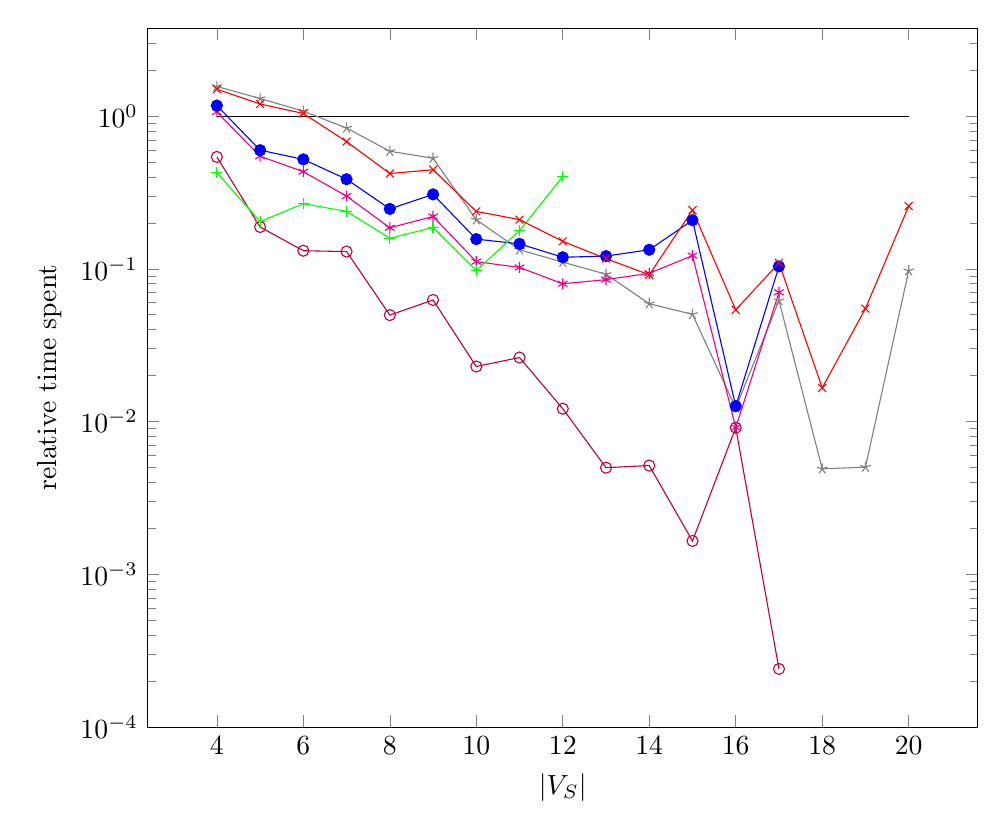
\begin{tikzpicture}
    \begin{axis}[
        xlabel=$|V_S|$,
        ylabel=relative time spent,
        ymode=log,
        legend style={at={(0.9,0.1)},anchor=south east},
        width=\textwidth,
		y tick label style={/pgf/number format/sci},
    ]


\addplot [mark=none, black] plot coordinates {
        (4,1) (20, 1)};
%\addlegendentry{No contraction}

	
	\addplot[
        mark=o,
        purple,
    ] plot coordinates {
        (4,0.5406515860434231)
        (5,0.18785238621358155)
        (6,0.1313898693246026)
        (7,0.12968087426224423)
        (8,0.04975578786006005)
        (9,0.06250441621787829)
        (10,0.02291763153069323)
        (11,0.026239199263713514)
        (12,0.012116839676172384)
        (13,0.004980595524332248)
        (14,0.005144230579578944)
        (15,0.0016492435304128457)
        (16,0.009108127743934116)
        (17,2.39411472197788E-4)
};
%    \addlegendentry{GDFS O IP}

\addplot[
        mark=star,
        gray,
    ] plot coordinates {
        (4,1.564264576045)
        (5,1.3044268948002964)
        (6,1.0779187100450964)
        (7,0.835982515879533)
        (8,0.5891175637322107)
        (9,0.5296276854812295)
        (10,0.20943673532574508)
        (11,0.1332559624097141)
        (12,0.11055593973933432)
        (13,0.09214123221094588)
        (14,0.05906133105316621)
        (15,0.05030047639103612)
        (16,0.012261524417415466)
        (17,0.06190271276571946)
        (18,0.004891557464661643)
        (19,0.005023467236129495)
        (20,0.09721129856411416)
};
%    \addlegendentry{GDFS C}


\addplot[
        mark=asterisk,
        magenta,
    ] plot coordinates {
        (4,1.0647032384996173)
        (5,0.5464303184358585)
        (6,0.43259746830858214)
        (7,0.29933523278634744)
        (8,0.185683374814357)
        (9,0.22002307269535923)
        (10,0.11140520704714015)
        (11,0.10205941312301019)
        (12,0.0797883687267593)
        (13,0.08491982151584633)
        (14,0.09342236316366812)
        (15,0.12200531503514861)
        (16,0.009112353995585515)
        (17,0.07011738991519775)
};
%    \addlegendentry{GDFS A IP}


\addplot[
        mark=*,
        blue,
    ] plot coordinates {
        (4,1.1732008189190344)
        (5,0.5987836864801016)
        (6,0.5208779931571201)
        (7,0.3863511956599727)
        (8,0.24675777694478437)
        (9,0.3072586029941962)
        (10,0.15645774275452057)
        (11,0.14567516195730124)
        (12,0.11902720146666647)
        (13,0.12115498638742035)
        (14,0.1332611638337713)
        (15,0.20805857181266843)
        (16,0.012601727180247312)
        (17,0.10371121285669947)
};
%    \addlegendentry{K-Path}

\addplot[
        mark=+,
        green,
    ] plot coordinates {
        (4,0.4269404047456055)
        (5,0.20382248417977045)
        (6,0.2669423065984091)
        (7,0.2379083813426592)
        (8,0.15878409767837634)
        (9,0.18627099036241238)
        (10,0.09728713629116212)
        (11,0.17771427973978168)
        (12,0.4025575819836778)
};
%    \addlegendentry{CP}
	
	\addplot[
        mark=x,
        red,
    ] plot coordinates {
        (4,1.5016288184210713)
        (5,1.2006306704032468)
        (6,1.0411914932334647)
        (7,0.6807867382482929)
        (8,0.42113301579781187)
        (9,0.4454296971733875)
        (10,0.23775196252967973)
        (11,0.2099983957550243)
        (12,0.15124037808888813)
        (13,0.1166188474735059)
        (14,0.09139802130807367)
        (15,0.24260975460559725)
        (16,0.053826733086807126)
        (17,0.10922977681106211)
        (18,0.016610936461570726)
        (19,0.054963613128898324)
        (20,0.25771949929195687)
};
%    \addlegendentry{DFS}
	


%\addplot[
%        mark=x,
%        red,
%    ] plot coordinates {
%        (4,1.1732605514536567)
%        (5,1.196916188570318)
%        (6,1.1785456812485087)
%        (7,0.9954870013054639)
%        (8,3.525437510655584)
%        (9,1.4492110968852605)
%        (10,1.747381055099775)
%        (11,2.2270690506062127)
%        (12,1.2853934585525963)
%        (13,2.4238390071533145)
%        (14,1.3323905497689534)
%        (15,1.9053869795283003)
%        (16,0.48107044214796724)
%        (17,2.689105479333416)
%        (18,1.6898544382126748)
%        (19,0.9452484856043308)
%        (20,0.7898504601171549)
%        (21,0.08308472050964744)
%        (22,0.010893076925442502)
%        (23,0.1812527204673673)
%        (24,0.05728059082927839)
%        (25,5.443902225728544)
%};
%    \addlegendentry{DFS}


%\addplot[
%        mark=o,
%        purple,
%    ] plot coordinates {
%        (4,0.5520630930461605)
%        (5,0.3167780166100581)
%        (6,0.15039692039595431)
%        (7,0.24510767406414147)
%        (8,0.38213533186187054)
%        (9,0.3108804215985045)
%        (10,0.1807787773743944)
%        (11,0.3299920410160406)
%        (12,0.19012573181575232)
%        (13,0.24472040784270033)
%        (14,0.19143954341561553)
%        (15,0.6627219343829152)
%        (16,0.005733506512017317)
%        (17,3.023867931706281E-4)
%};
%    \addlegendentry{GDFS O IP}


%\addplot[
%        mark=star,
%        gray,
%    ] plot coordinates {
%        (4,2.4400816563321017)
%        (5,1.633197217665063)
%        (6,1.2185290307235452)
%        (7,0.9546648292258212)
%        (8,1.728111058353678)
%        (9,0.9769781523573012)
%        (10,0.6904942121852058)
%        (11,4.816564314417738)
%        (12,0.6783371965634181)
%        (13,4.011191995338261)
%        (14,0.7170173730516766)
%        (15,1.5965119303548203)
%        (16,0.23663227697171496)
%        (17,0.5542490660149222)
%        (18,0.3058591166536577)
%        (19,0.7018097729480665)
%        (20,0.27875622792926213)
%        (21,1.1344734954273632)
%        (22,0.028755331201753886)
%        (23,0.0777791424367319)
%};
%    \addlegendentry{GDFS C}


%\addplot[
%        mark=*,
%        blue,
%    ] plot coordinates {
%        (4,1.2419213216803755)
%        (5,0.8200821368474451)
%        (6,0.5765214516413038)
%        (7,0.565346845113148)
%        (8,1.3724712483006076)
%        (9,1.0626551826303774)
%        (10,0.8227740807006784)
%        (11,3.6735922630894127)
%        (12,1.3221239755232121)
%        (13,5.700758822957509)
%        (14,3.5989514748969498)
%        (15,1.8366783161451987)
%        (16,0.5267585376114875)
%        (17,0.8256958007787268)
%        (18,1.4987328025927649)
%        (19,0.08315275360896346)
%        (20,0.7615106824048338)
%        (21,0.2227706812823126)
%};
%    \addlegendentry{K-Path}
%	\addplot[
%        mark=+,
%        green,
%    ] plot coordinates {
%        (4,0.6251754120590031)
%        (5,0.7127354515628973)
%        (6,0.5384995648933136)
%        (7,0.4718614006762697)
%        (8,0.7587386430883546)
%        (9,0.6801119660951308)
%        (10,0.7579067651040344)
%        (11,0.6568766478712005)
%        (12,1.2358097901656984)
%};
%    \addlegendentry{CP}

%\addplot[
%        mark=asterisk,
%        magenta,
%    ] plot coordinates {
%        (4,1.0218394225281529)
%        (5,0.7182128970849538)
%        (6,0.48051752660220404)
%        (7,0.431379262711197)
%        (8,1.139769610563402)
%        (9,0.6462462777019891)
%        (10,0.4984166569477635)
%        (11,2.3191988060404114)
%        (12,0.600719665743818)
%        (13,1.9928831703649212)
%        (14,0.5997476794608112)
%        (15,2.3702852860015766)
%        (16,0.2501718737108647)
%        (17,1.963031760531809)
%        (18,0.7865261017018875)
%        (19,0.6636357792814185)
%        (20,0.4302617051584967)
%        (21,0.11666290941349455)
%        (22,0.03731454564481351)
%        (23,0.18654788991103444)
%};
%    \addlegendentry{GDFS A IP}

	
	
    \end{axis}
    \end{tikzpicture}

\caption{$|V_T|=3|V_S|$}
\end{subfigure}\\[1ex]
\begin{subfigure}{0.5\linewidth}
\centering

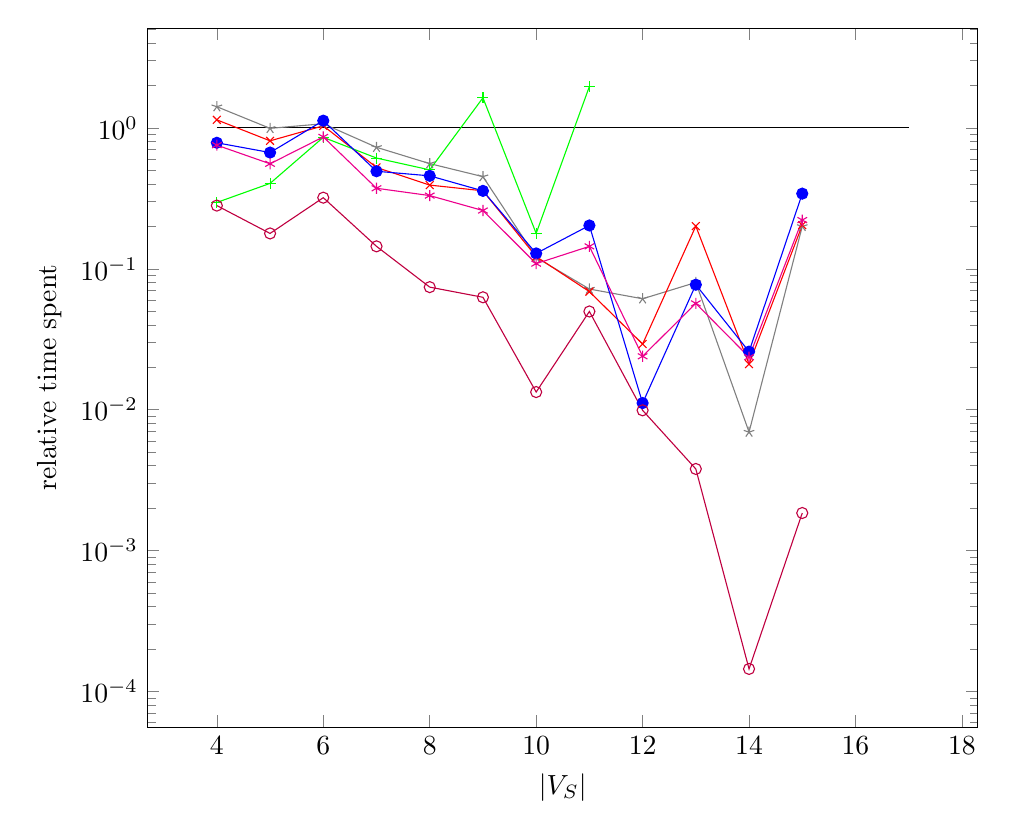
\begin{tikzpicture}
    \begin{axis}[
        xlabel=$|V_S|$,
        ylabel=relative time spent,
        ymode=log,
        legend style={at={(0.9,0.1)},anchor=south east},
        width=\textwidth,
		y tick label style={/pgf/number format/sci},
    ]


\addplot [mark=none, black] plot coordinates {
        (4,1) (17, 1)};
%\addlegendentry{No contraction}

	\addplot[
        mark=star,
        gray,
    ] plot coordinates {
        (4,1.4150313228372156)
        (5,0.9931089780372052)
        (6,1.0711893924147513)
        (7,0.7287433844993442)
        (8,0.5580336822334304)
        (9,0.45098800643949294)
        (10,0.12035734271971275)
        (11,0.07185662459924363)
        (12,0.061270869720004735)
        (13,0.07996994856322678)
        (14,0.0069337049664659365)
        (15,0.19997291246935858)
};
%    \addlegendentry{GDFS C}

\addplot[
        mark=x,
        red,
    ] plot coordinates {
        (4,1.1414201843876104)
        (5,0.809932163821809)
        (6,1.035209481616773)
        (7,0.524271062265468)
        (8,0.39302087430090826)
        (9,0.3578043691511488)
        (10,0.12214201172912188)
        (11,0.06885304754889712)
        (12,0.029241866518748955)
        (13,0.20088131729557912)
        (14,0.02106421225202191)
        (15,0.2041959874232657)
};
%    \addlegendentry{DFS}


\addplot[
        mark=+,
        green,
    ] plot coordinates {
        (4,0.2957715422588946)
        (5,0.4039693151705631)
        (6,0.8576103567062523)
        (7,0.611136842539274)
        (8,0.5039078563666931)
        (9,1.6368759420585266)
        (10,0.17838843269084026)
        (11,1.9695600715158896)
};
%    \addlegendentry{CP}

\addplot[
        mark=*,
        blue,
    ] plot coordinates {
        (4,0.7847268248450774)
        (5,0.6687217050275467)
        (6,1.1261548415934364)
        (7,0.4925445033611991)
        (8,0.45704298044965924)
        (9,0.35742057060947313)
        (10,0.128612015175269)
        (11,0.20308934398456394)
        (12,0.011139696619114561)
        (13,0.07711180448206871)
        (14,0.025822554979476078)
        (15,0.3417612423571849)
};
%    \addlegendentry{K-Path}

\addplot[
        mark=asterisk,
        magenta,
    ] plot coordinates {
        (4,0.7547769389469375)
        (5,0.5565971887626566)
        (6,0.8633572665036556)
        (7,0.37305369668133204)
        (8,0.3309908929077787)
        (9,0.25924812346158027)
        (10,0.10882869144475564)
        (11,0.1443116551616309)
        (12,0.02393540782562589)
        (13,0.056815118476015725)
        (14,0.02359541092466829)
        (15,0.22173612580802898)
};
%    \addlegendentry{GDFS A IP}


\addplot[
        mark=o,
        purple,
    ] plot coordinates {
        (4,0.2810473555343349)
        (5,0.1782672123525788)
        (6,0.319850284994006)
        (7,0.14437026097789094)
        (8,0.07412250627959217)
        (9,0.06277787793471931)
        (10,0.013337293008856575)
        (11,0.04979135381171951)
        (12,0.009893636551485722)
        (13,0.0037954716122957726)
        (14,1.4440290497311895E-4)
        (15,0.0018470151154413993)
};
%    \addlegendentry{GDFS O IP}



%  \addplot[
%        mark=x,
%        red,
%    ] plot coordinates {
%        (4,0.8783007924961822)
%        (5,1.9866466250704127)
%        (6,46.23915298831981)
%        (7,1.9286013087935467)
%        (8,0.22144887888388298)
%        (9,0.6073880518853707)
%        (10,0.9499470941285778)
%        (11,0.3071513116204406)
%        (12,0.20181763488775617)
%        (13,0.5247142961355576)
%        (14,0.08240035713162575)
%        (15,1.3331646694970158)
%        (16,0.030153907349204312)
%        (17,0.7818188550294238)
%};
%     \addlegendentry{DFS}

%    \addplot[
%        mark=o,
%        purple,
%    ] plot coordinates {
%        (4,0.13253526170374963)
%        (5,0.340135432164708)
%        (6,1.790446045629151)
%        (7,0.21172911942986739)
%        (8,0.00939924729361108)
%        (9,0.1386409264007632)
%        (10,0.15954167221271842)
%        (11,0.05059726207816495)
%        (12,0.04218464066556149)
%        (13,0.011328653011651979)
%};
%    \addlegendentry{GDFS O IP}

% \addplot[
%        mark=star,
%        gray,
%    ] plot coordinates {
%        (4,1.6271054568492918)
%        (5,1.2019347721569387)
%        (6,22.57207288783596)
%        (7,1.60714000055505)
%        (8,0.41137411151774583)
%        (9,0.5862167248296255)
%        (10,0.7637400611154803)
%        (11,0.356373039522627)
%        (12,0.17288151392047257)
%        (13,0.48433813085979627)
%        (14,0.046838546665677216)
%        (15,1.5140584943694408)
%        (16,0.07823427303666675)
%        (17,1.8750942580464485)
%};
%    \addlegendentry{GDFS C}


%\addplot[
%        mark=*,
%        blue,
%    ] plot coordinates {
%        (4,0.60298022841694)
%        (5,1.0316944681766402)
%        (6,15.991061194154563)
%        (7,1.063190444555428)
%        (8,0.08058508916228702)
%        (9,3.019451686125926)
%        (10,0.79704175618652)
%        (11,4.998970774016183)
%        (12,0.06678499576131569)
%        (13,0.5580121902125518)
%        (14,0.08746647794145956)
%        (15,1.0672969432977613)
%        (16,0.23788697499741307)
%};
%    \addlegendentry{K-Path}

%   \addplot[
%        mark=+,
%        green,
%    ] plot coordinates {
%        (4,0.2760410688096132)
%        (5,0.7968662246398364)
%        (6,1.6383115468640344)
%        (7,0.5747225278886098)
%        (8,0.16947067443329888)
%        (9,9.48379348911334)
%        (10,0.04037684393142793)
%};
%    \addlegendentry{CP}
%	\addplot[
%        mark=asterisk,
%        magenta,
%    ] plot coordinates {
%        (4,0.5669029018884123)
%        (5,0.8690518164754274)
%        (6,16.40156998152306)
%        (7,0.7704428785494475)
%        (8,0.07028167075789626)
%        (9,0.4575408842013087)
%        (10,0.38859339371640744)
%        (11,0.31086090173433223)
%        (12,0.0424840967267095)
%        (13,0.5265194610065892)
%        (14,0.02960328686421898)
%        (15,0.8762590796270182)
%        (16,0.1859213565027673)
%        (17,0.42289838038406646)
%};
%    \addlegendentry{GDFS A IP}

	
	
    \end{axis}
    \end{tikzpicture}

\caption{$|V_T|=5|V_S|$}
\end{subfigure}
\begin{subfigure} {0.5\linewidth}
\centering

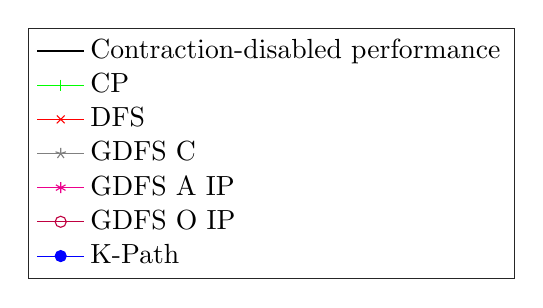
\begin{tikzpicture} 
    \begin{axis}[%
    hide axis,
    xmin=10,
    xmax=50,
    ymin=0,
    ymax=0.4,
    legend style={draw=white!15!black,legend cell align=left}
    ]
	\addlegendimage{black}
    \addlegendentry{Contraction-disabled performance}; 
     
    \addlegendimage{green, mark=+}
    \addlegendentry{CP};
    
    \addlegendimage{red, mark=x}
    \addlegendentry{DFS};
    
    \addlegendimage{gray, mark=star}
    \addlegendentry{GDFS C};
    
    \addlegendimage{magenta, mark=asterisk}
    \addlegendentry{GDFS A IP};
    
    \addlegendimage{purple, mark=o}
    \addlegendentry{GDFS O IP};
    
    \addlegendimage{blue, mark=*}
    \addlegendentry{K-Path};
    
    \end{axis}
\end{tikzpicture}

\end{subfigure}

\caption{Mean relative time consumption of contraction-enabled subgraph homeomorphism search compared to contraction-disabled for different path iteration methods. For data points below the reference line contraction saves time while for data points above it contraction costs extra time. We handled a maximum of 1000 test cases or 10 minutes per value of $|V_S|$ for each path iteration method.}	
\label{fig:contraction-performance}
\end{figure}
